\section{Introduction}
The advancements of quantum technologies in  recent years have brought the focus of the scientific community on the need to investigate novel approaches to produce more compact and stable quantum devices.
While the progressive miniaturisation of the devices poses geometrical constraints on the system, an optimal level of control on the quantum particles is required.
Waveguides in particular play a crucial role in the confinement and transmission of quantum states in a wide variety of experiments where the control is usually achieved by increasing the intensity of the trapping.
This approach is clearly energy consuming so it would be advisable to design protocols relying primarily on the geometry of the waveguide and only subsequently focusing on the strength of the trapping.
The effects of the geometry on waveguides are well known and could be quite disrupting as - for example - it has been shown that even the slightest bending in waveguides results in the production of bound states \cite{BoundStatesInGoldst1992}.
Historically, studies relied on the adiabatic approximation, by virtue of which the curvature is supposed to vary gently.
The adiabatic approximation is ineffective in those systems where strong geometrical constraints are in place as, for instance waveguides with sharp bendings \cite{BoundStatesInClark1996, BoundStatesInBittne2013, MultipleBoundCarini1993}.
Recently, the surge of inverse engineered protocols under the name of Shortcuts to Adiabaticity  \cite{ShortcutsToAdGuery2019} (STA) has proven to be extremely effective in systems where the adiabatic approach is deemed to be unapplicabile.
STA offer a framework to control the evolution of a system starting in some initial state to obtain the desired final state by ensuring that selected external parameters meet the boundary conditions.
In the context of waveguides, Gu\'ery-Odelin et al. in the seminal paper \cite{QuantumControlImpens2020} have applied the approach based on STA to design the curvature of sharply bent waveguides to minimise the loss of coherence in travelling quantum particles with excellent results.
The range of applicability of this protocol extends to all systems where matter-wave circuits are employed.
One of the most relevant example of application is atomtronics \cite{RoadmapOnAtomAmico2021}, an emerging field where the information carriers are cold neutral atoms and the applications of which span from quantum interferometry \cite{MagneticallyGuQiLu2017, 80kmomentumSeMcdona2013} to quantum circuital elements \cite{FocusOnAtomtrAmico2017, AdvancesInAtoPepino2021}.
The approach in \cite{QuantumControlImpens2020} is based on the assumption that - in first approximation - a quantum particle can be modelled as a classical one and that by imposing the trajectory it is possible to inverse engineer the curvature satisfying the boundary conditions.
In this paper we will first briefly review the STA-based approach of Gu\'ery-Odelin et al. and we subsequently change the controlling parameters to further investigate the validity of the protocol when the classical approximation loses its validity.
\section{Hamiltonian of a bent waveguide}
Let us consider a system composed by a waveguide where the confinement is achieved by means of a harmonic trapping of intensity $ \omega $.
With no loss of generality, we can assume that the waveguide is formed by two straight ducts forming an angle $\alpha = \pi/2$ and connected by a bent section.
We also assume that the initial state is a separable 2D Gaussian wave packet entering the curved trait with momentum $k_0$, and hence it can be written as 
\begin{align}
\label{eq:initial_state}
	\psi_{0}(x,y) = \left(\frac{1}{2 \pi \sigma_{x}^{2}}\right)^{1/4}\exp\left(- \frac{x^{2}}{4\sigma_{x}^{2}} - i k_{0}x  \right)\\
	\left(\frac{1}{2\pi\sigma_{y}^{2}}\right)^{1/4}\exp\left(-\frac{y^{2}}{4\sigma_{y}^{2}}\right)
\end{align}
where $ \sigma_{y} $  is the dispersion along the transverse axis equal to $\sqrt{\hbar/2 m \omega}$ while the longitudinal dispersion $ \sigma_{x} $ is set.
If no bending was involved, $\psi_0$  would evolve under the effect of the Hamiltonian of a straight waveguide 
\begin{equation}
	\label{eq:straightwave}
	 H = -\frac{\hbar^2}{2m} \left(\partial_{x}^{2} + \partial_{y}^{2}\right) + \frac{1}{2}m\omega^2y^2
\end{equation}
and we could write the wave function at the time $t$ as the product of a free particle along $x$ and the ground state of the harmonic oscillator along $y$. 
On the other hand, if we assume the waveguide to be bent and considering the bottom of the trap to follow a curve $\Ga$ in $\mathbb{R}^2$, the modification in the geometry of the system produces mixing between the two components of the wave function, hence making harder it to control the particle.
The Hamiltonian of this system has been studied extensively in the literature (see for example \cite{TheEffectiveHKrejci2012}) and can be evaluated by using the most convenient curvilinear coordinates $(s,u)$ where $s$ is defined as the arc length of $\Ga$ defined as $s(t) = \int_0^t d\tau||\Ga'(\tau)||$ and $u$ is the transverse coordinate.
The local coordinate axis are the normal vectors \textbf{t}(s), \textbf{n}(s), with \textbf{t} the tangent vector to the curve and \textbf{n} the unit vector perpendicolar to \textbf{t} as in  \cref{fig:setup}.
\begin{figure}
	%(a)	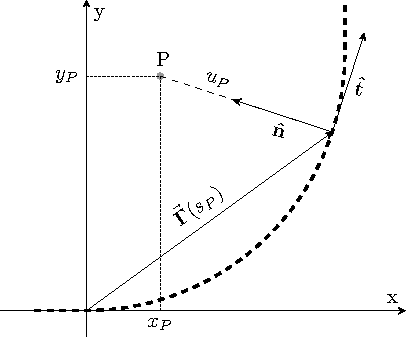
\includegraphics[width = .7\columnwidth]{gfx/frenet.pdf}\\
		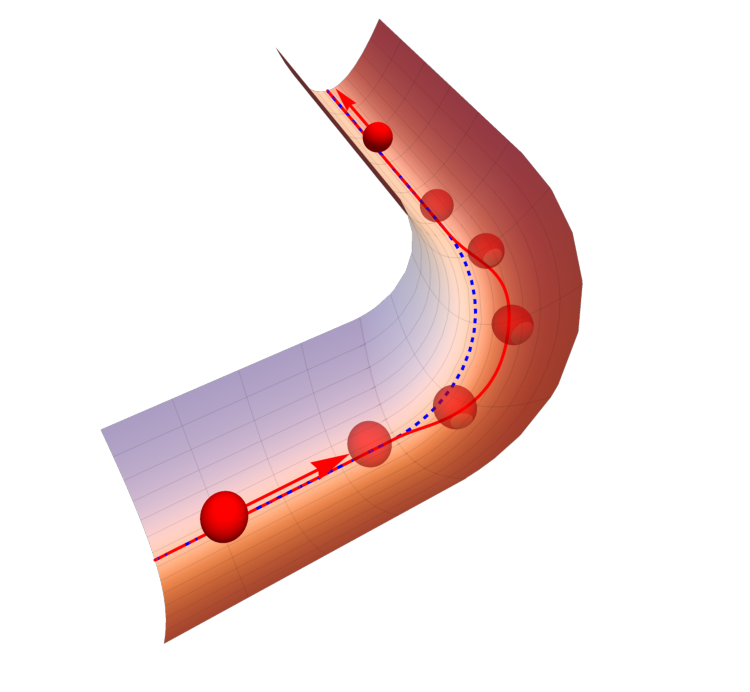
\includegraphics[width = .7\columnwidth]{gfx/tube.pdf}
		\caption{%(a) Schematic to show the construction of the Frenet Serrat frame of reference and how the curvilinear coordinates are defined.\\
		 Example of the imposed trajectory of the particle in a waveguide with harmonic trapping}
		\label{fig:setup}
\end{figure}
With this prescriptions, the coordinate transformation from Cartesian coordinates to the so-called Frenet Serrat frame can be written as $(x(s,u), y(s,u)) = \Ga(s)  + u \mathbf{n}(s) $ as in \cref{fig:setup}.
Moreover, the following relations hold and they are called Frenet Serrat equations:
\begin{align}
	\diff{\Ga(s)}{s}  &= \mathbf{t}(s) \label{eq:frenet1}\\ 
	\diff{\mathbf{t}(s)}{s}  &= \gamma(s)\mathbf{n}(s) \label{eq:frenet2}\\ 
	\diff{\mathbf{n}(s)}{s}  &= -\gamma(s)\mathbf{t}(s) \label{eq:frenet3}
\end{align}
where $\gamma(s)$ is the curvature of $\Ga$ and it is invariant under transformation.
The curvature $\gamma$ is the most relevant quantity in this case since the Hamiltonian of the system can be written as 
\begin{equation}
	\label{eq:curvedhamilton}	
	H = - \frac{\hbar^2}{2m} \left( \partial_s \frac{1}{(1-\gamma)^2} - \partial_{u}^{2}\right)
	+ \frac{1}{2} m\omega^2u^2 + V(s,u)
\end{equation}
where $V(s,u)$ is the attractive potential resulting from the change of coordinates 
\begin{equation}
	\label{eq:potential}
	V(s,u) = -\frac{\gamma^2}{4(1-u\gamma)^2} - \frac{u\ddot{\gamma}}{2(1-u\gamma)^3} -\frac{5}{4}\frac{u^2\dot{\gamma}^2}{(1-u\gamma)^4}.
\end{equation}
In many studies an adiabatic approach has been followed to solve the Hamiltonian \eqref{eq:curvedhamilton} 
Adiabatic in the sense that the curvature has been chosen to be varying slowly with respect ot the $s$ coordinate, i.e. $\dot{\gamma}, \ddot{\gamma} \approx 0 $.
This approach does not take into account many particular settings, for example the ones with geometric consstraints where a sharp turn needs to be considered.
For this reason Gu\'ery-Odelin et al in \cite{QuantumControlImpens2020} have designed a semi-classical protocol based on Shortcuts to Adiabaticity (STA) to circumvent the limitations of the adiabatic approach.
In \cite{QuantumControlImpens2020} the curvature $\gamma$ has been inversed engineered by writing the classical 2D Newton's equations of motion for a particle with initial speed $\dot{s}_0$.
The idea is to impose the dependence of the curvature coordinates $(s,u)$ from the time parameter $t$ so that the position of a point particle of mass $m$ can be described bt the vector $\Ga(s(t))$.
We can hence write the respective Newton's equation in vector form as 
\begin{equation}
	\label{eq:newtfirstlaw}
	m \diff[2]{\Ga(s(t))} t = - \nabla V_\perp (u)
\end{equation}
where $ V_\perp(u) $ is the conservative trapping potential that in curvilinear coordinates simply becomes $ \frac{1}{2}\omega^2 u^2 $.
The solution of \eqref{eq:newtfirstlaw} is obtained by making use of \crefrange{eq:frenet1}{eq:frenet3} and projecting the resulting vector onto the two coordinate axis \textbf{t} and \textbf{n}:
\begin{align}
	& \ddot{s} (1-u\gamma)  -\dot{s}(2\dot{u}\gamma + u \dot{\gamma}) + \frac{1}{2}\omega^2u^2 = 0 \\
	& \ddot{u} + \omega^2u + \dot{s}^2\omega(1-u\gamma)  = 0.
\end{align}
Furthermore, the conservation of energy can be written as $\frac{1}{2}\left(\diff{\Ga}{t}\right)^2 + V_\perp(s,u) = E$ or, equivalently
\begin{equation}
	\label{eq:energyconserve}
	\dot{u}^2 + \omega^2u^2 + \dot{s}^2(1-u\gamma)^2 = \dot{s}_0^2.
\end{equation}
By setting $ v_\gamma = \dot{s}(1-u\gamma)   $, it has been shown that it is possible to retrieve $ \gamma $ using the following formula
\begin{equation}
	\label{eq:stacurvature}
	\gamma = \frac{\dot{v}_\gamma}{\diff{}{t}(uv_\gamma)}	,
\end{equation}
hence the curvature can be obtained only by fixing the transverse trajectory $ u_{sta}(t) $ as exemplified in \cref{fig:setup}.
The resulting curvature $ \gamma_{sta} $ can then be used as the groundwork to numerically solve the Hamiltonian \eqref{eq:curvedhamilton} and thest the performances of the waveguide's geometry also in quantum settings.
It has already been shown in \cite{QuantumControlImpens2020} that a curve obtained following this procedure provides a higher level of fidelity when  compared to a circular waveguide of radius $R$.
In the following we will try ot continue on these tracks by testing different transverse trajectories.
